% !TEX root = main.tex

\chapter{試料構造と測定方法}
%\label{chap:simulation}

\section{はじめに}

\section{試料作製}
\subsection{試料構造}
\subsection{ブロードコンタクトレーザー}
\subsection{リッジ導波路型レーザー}
\subsection{マウント(ダイボンディング??)}
\section{測定方法}
本研究ではエピウエハの品質評価のための測定と利得スイッチング動作を起こしデバイスの高速特性を評価するための測定を行った。
\subsection{IL}
\begin{figure}[htbp]
	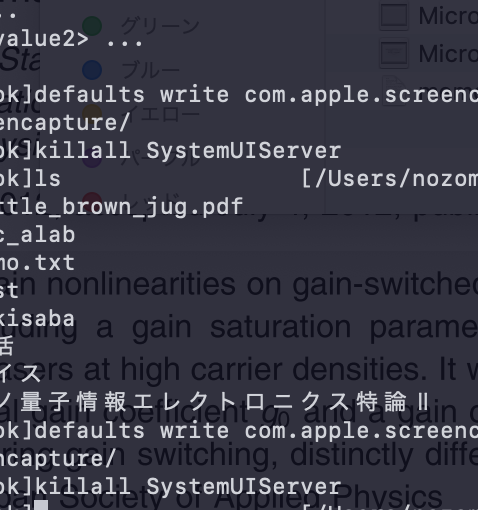
\includegraphics[width=15cm]{./test_fig.png}
	\caption{test}
\end{figure}
\subsection{電流注入利得スイッチング実験}
